% Formato para un capítulo cualquiera

%Título del capítulo
\chapter{Interface RestFul} 

\section{Introducción}
En este capítulo se explicarán todas las estructuras que se han diseñado para los accesos a datos de la base de datos \textbf{SocialNetwork} a través de \textbf{Servicios Web}. Todas estas estructuras se han almacenado en una API pública para que, posteriormente a este desarrollo, cualquier programador que quiera hacer uso de dicha base de datos pueda hacerlo de forma transparente accediendo únicamente a los objetos que quiere referenciar, tal y como se han diseñado otras bases de datos, tales como la que utiliza Facebook para acceder al perfil de un usuario determinado.
\bigskip
\par
En los primeros capítulos del presente documento se estableció la definición de \textbf{Servicios REST}, que no son más que Servicios Web que se basan en protocolos HTTP como medio de obtención de datos. Todo Servicio REST se basa en el concepto de ``Todo recurso(información) debe tener y ser accesible mediante una URI única''. Para realizar este acceso, se usan las operaciones restringidas únicamente a los métodos GET, PUT, POST y DELETE, que pasaremos a explicar a continuación:
\bigskip
\par
\begin{enumerate}
\item Método \textbf{GET}: Este método accede a un recurso determinado y devuelve un objeto como respuesta con todos los datos asociados al recurso. Su respuesta puede ser tratada mediante XML o JSON, a gusto del desarrollador.
\item Método \textbf{POST}: Este método introduce en la base de datos un recurso en la direción URI que se le indique. Internamente, cuando la petición llega al proceso que gestiona internamente la base de datos remota, éste realiza una operación \textbf{INSERT} hacia todas las tablas que sean referenciadas por el objeto que se le ha pasado al argumento de llamada. Cuando éstos datos sean inconsistente, la base de datos no realizará operación alguna y se devolverá un código de error.
\item Método \textbf{PUT}: Análogamente al método POST, este método hará una actualización de un recurso en base de datos, realizando una operación \textbf{UPDATE} en la base de datos remota cuando ésta reciba la petición y el objeto que se desea actualizar. Al igual que el método anterior, si los datos no son consistentes se devolverá un error al método que realiza la llamada.
\item Método \textbf{DELETE}: Este método elminará el recurso que apunta a la URI que se ha referenciado. 
\end{enumerate}
Todos los métodos anteriores devuelven códigos de error HTTP que serán tratados en capítulos posteriores.
\bigskip
\par
Para realizar esta comunicación entre aplicación que demanda datos, Interfaz RestFul y base de datos, internamente vamos a necesitar las siguientes estructuras:
\begin{enumerate}
\item Una base de datos desarrollada bajo cualquier tecnolgía, en nuestro caso, sobre el entorno MySQL 5.
\item Un proyecto que gestione internamente todas las operaciones de base de datos y ofrezca servicios RestFul a los datos y que, a su vez, puedan ser acessibles mediante éstos servicios.
\item Una interfaz RestFul definida para el acceso a datos que apunte directamente a todos los servicios definidos internamente por el proyecto que gestiona la base de datos.
\end{enumerate}
\bigskip
\par
En éste capítulo se pasará a explicar cada una de estas estructuras y a definir todos los servicios necesarios para esta arquitectura, mostrada en la imagen \ref{ArqServRestFul}.
\begin{figure}
\begin{center}
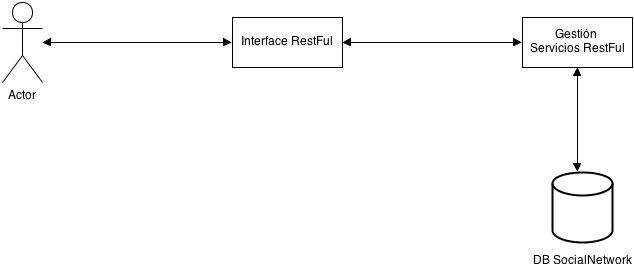
\includegraphics[width=8cm,height=4cm]{Figuras/ArqServRestFul.png}
\end{center}
\caption{\label{ArqServRestFul} Arquitectura de la Interface RestFul}
\end{figure}

\section{Casos de uso para la Interface RestFul}
En éste apartado, vamos a estudiar, mediante el diagrama de casos de uso mostrado en la imagen \ref{imgCasosUsoRestFul}, las posibles acciones a las que se enfrentará y para las que está diseñada la Inteface RestFul y el resto de componentes que necesita para interactuar.
\begin{figure}[h]
\begin{center}
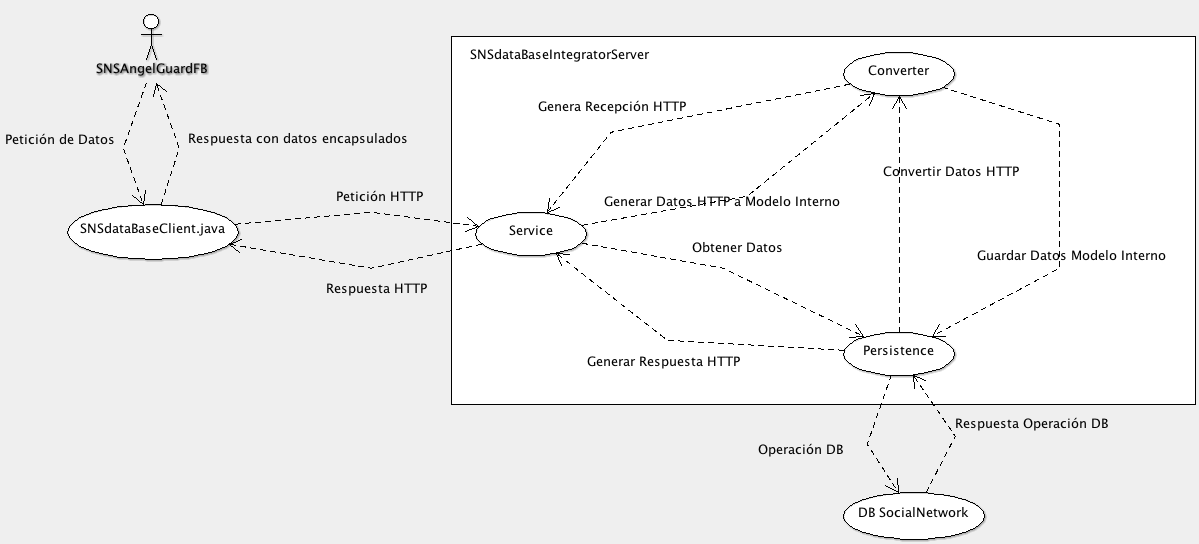
\includegraphics[width=17cm,height=11cm]{Figuras/imgCasosUsoRestFul.png}
\end{center}
\caption{\label{imgCasosUsoRestFul} Diagrama de Casos de Uso de la Interface RestFul}
\end{figure}
\bigskip
\par
El diagrama de casos de uso seguirá la siguiente secuencia:
\begin{enumerate}
\item La aplicación \textbf{SNSAngelGuardFB} generará una operación de datos, bien sea de petición, de actualización o de eliminación. A ésta petición irán encapsulados todos los datos necesarios para realizarla y la URI correspondiente al objeto que se quiere añadir, actualizar o eliminar de la base de datos.
\item La clase \textbf{SNSdataBaseClient.java} generará la operación HTTP necesaria para la operación y la enviará via HTTP al proyecto que se encargará de gestionar los Servicios RestFul junto con las operaciones con la base de datos, en última instancia. La clase SNSdataBaseClient.java contendrá una serie de métodos a los que se invocará para acceder a dichos servicios. Esta será nuestra Interface RestFul en la práctica, ya que será la encargada de los envíos mediante las operaciones HTTP mencionadas anteriormente y de la recepción de las respuestas generadas encapsulando éstas en los tipos de datos necesarios para ser tratadas.
\item Cuando se invoca uno de los métodos de la clase SNSdataBaseClient.java, se envia la petición HTTP al proyecto \textbf{SNSdataBaseIntegratorServer}, quien será el encargado de interactuar con la base de datos. Este proyecto se substenta sobre tres pilares básicos:
\begin{enumerate}
\item El paquete \textbf{service} contendrá, para cada recurso, las clases necesarias que son las que ofrecen los Servicios RestFul que son invocados por la Interface, es decir, cada método que se invoca tiene una entrada en estas clases. Serán las encargadas de recepcionar la petición, analizar mediante la URI recibida a qué objeto se refiere y se debe tratar y, finalmente, enviar la respuesta de la operación.
\item Cuando llega una petición, bien sea de consulta o de actualización, se deberán parsear los datos recibidos de la operación al modelo interno de análisis. Estas operaciones serán realizadas por el paquete \textbf{converter} el cual, para cada recurso de la base de datos, tendrá una serie de estructuras que recibirán los datos de la petición HTTP y los convertirán a datos internos para que puedan ser procesados.
\item Tras realizar el parseo conveniente de los datos, éstos serán enviados a la clase que corresponda, según el recurso, del paquete \textbf{persistence}, el cual, para cada recurso de la base de datos, tendrá una serie de estructuras que serán, en último término, las encargadas de realizar la operación en base de datos y propagar la respuesta que a ésta se produzca, a su nivel superior, es decir, a la clase que corresponda del paquete \textbf{service}, el cual será capaz de propagarlo hasta la Interface RestFul.
\end{enumerate}
\item Una vez que la respuesta ha llegado, el método de la clase SNSdataBaseClient.java parseará el objeto al tipo de datos que se le haya indicado en la petición y propagará la respuesta a su nivel superior, es decir, al método de la aplicación SNSAngelGuardFB que lo haya invocado.
\item Finalmente, al llegar la respuesta al método que originó toda la operación, se analizará el código de respuesta, se obtendrán los datos en caso afirmativo y se continuará con la ejecución de la aplicación.
\end{enumerate}

\section{Projecto SNSdataBaseIntegratorServer}
\textbf{SNSdataBaseIntegratorServer} será el encargado de realizar toda la gestión de los servicios RestFul y, tras evaluar las peticiones, acceder a la base de datos SocialNetwork y realizar la operación que se ha enviado. Tras realizar la operación, generará una respuesta en la que irán encapsulados tanto los datos obtenidos como el código de respuesta HTTP(ver \textbf{Anexo \ref{appHttp}}).
\bigskip
\par
Este proyecto está realizado bajo el lenguaje de programación \textbf{Java} y ha sido desarrollado automáticamente por las herramientas de que dispone el entorno de desarrollo \textbf{NetBeans}, las cuales, a partir de una base de datos, en nuestro caso SocialNetwork, generan todos los Servicios RestFul y todas las estructuras necesarias para realizar la gestión de dicha base de datos. Con ésto conseguimos una gestión de la base de datos totalmente independiente y, además, la base de datos puede no estar en la misma máquina que el servidor que ejecuta la operación pero, por el contrario, siempre se deberá tener ejecutando en un servidor web el proyecto SNSdataBaseIntegratorServer para que puedan llevarse a cabo estas operaciones.
\bigskip
\par
Como bien se ha mencionado anteriormente, este proyecto cuenta con los siguientes paquetes:
\begin{enumerate}
\item Paquete \textbf{es.uah.cc.ie.service}: El cual contendrá todos los servicios RestFul de la base de datos.
\item Paquete \textbf{es.uah.cc.ie.converter}: El cual contendrá todas las estructuras necesarias para realizar la conversión de datos de modelo interno a operación HTTP y viceversa.
\item Paquete \textbf{es.uah.cc.ie.persistence}: El cual contendrá todas las estructuras necesarias para, en última instancia, resolver la operación de base de datos referenciada en el Servicio RestFul. 
\end{enumerate}
\bigskip
\par
La estructura de paquetes puede verse reflejada en la imagen \ref{imgPackageSNSdataBaseIntegratorServer}.
\begin{figure}[h]
\begin{center}
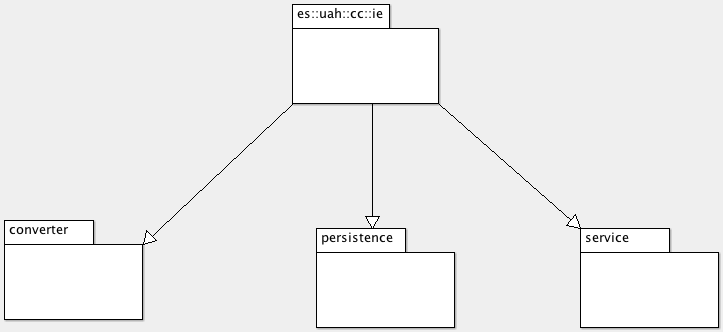
\includegraphics[width=10cm,height=5cm]{Figuras/imgPackageSNSdataBaseIntegratorServer.png}
\end{center}
\caption{\label{imgPackageSNSdataBaseIntegratorServer} Diagrama de paquetes del projecto SNSdataBaseIntegratorServer}
\end{figure}
Para cada recurso, cada paquete contendrá dos estructuras necesarias para su procesamiento( salvo el paquete \textbf{persistence}, que únicamente contendrá una clase por recurso), la estructura que procesa una unidad y la estructura que procesa un conjunto de unidades del mismo recurso. Por ejemplo, si queremos ver las estructuras necesarias para gestionar la tabla user, la imagen \ref{imgPackUser} nos despejará cualquier tipo de duda.
\begin{figure}[h]
\begin{center}
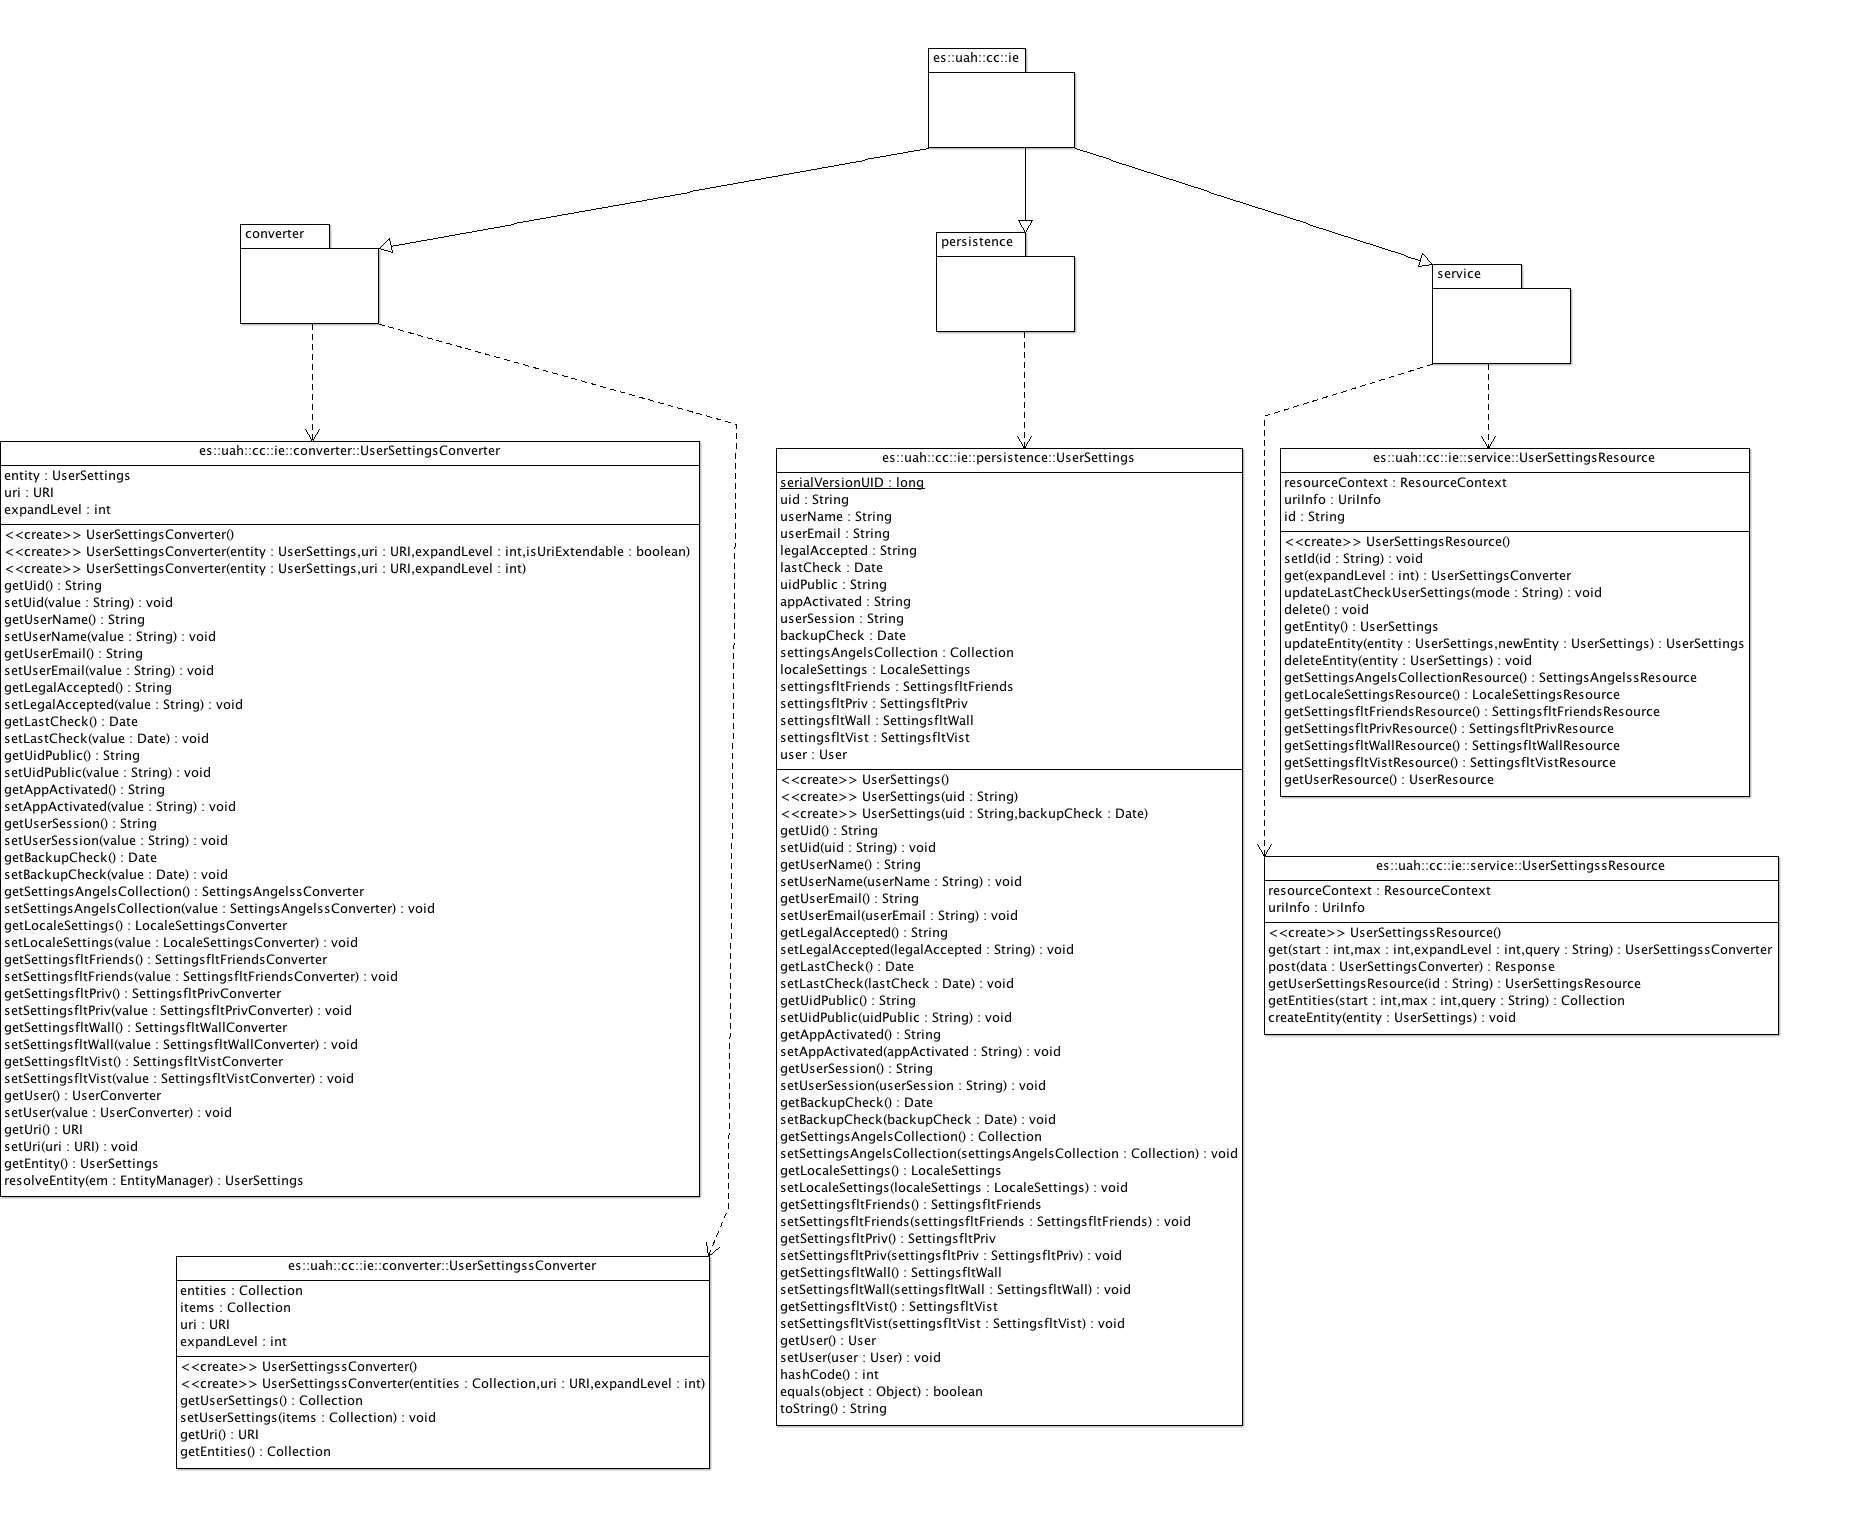
\includegraphics[width=18cm,height=15cm]{Figuras/imgPackUser.png}
\end{center}
\caption{\label{imgPackUser} Diagrama de clases para el recurso UserSettings}
\end{figure}

\subsection{Paquete es.uah.cc.ie.service}
Este paquete contendrá todo el soporte a una petición de un Servicio RestFul. En éste paquete se encontrará dos clases por cada recurso. La clase que gestiona una única entidad tendrá los siguientes componentes:
\begin{enumerate}
\item Atributo \textbf{ResourceContext}: Irá acompañado de la anotación \textbf{@Context}. Servirá para obtener el contexto en el que se está ejecutando el recurso y obtener su referencia física.\begin{verbatim}protected ResourceContext resourceContext;\end{verbatim} 
\item Atributo \textbf{UriInfo}: También irá acompañado de la anotación \textbf{@Context}. En él se almacenará la URI absoluta de acceso al recurso que se está procesando. \begin{verbatim}protected UriInfo uriInfo;\end{verbatim} 
\item Atributo \textbf{String id}: Almacenará el ID del objeto al que hace referencia dentro de la base de datos. \begin{verbatim}protected String id;\end{verbatim} 
\item Método \textbf{get}: Irá precedido de la anotación \textbf{@GET}. Obtendrá un objeto de la base de datos indicado por el parámetro \textbf{ExpandLevel}, que por defecto valdrá 1. Se podrá indicar, mediante la anotación \textbf{@Produces}, en qué formato se van a devolver los datos que ésta llamada produzca, en nuestro caso los datos se enviarán tanto en XML como en JSON, siendo éste último el formato elegido para la recepción.
\item Método \textbf{put}: Irá precedido de la anotación \textbf{@PUT}. Actualizará un determinado objeto de la base de datos. En éste caso, irá acompañado de la anotación \textbf{@Consumes}, que indicará al método qué tipo de datos va a recibir. En nuestro caso, podrá recibir tanto en formato XML como en JSON.
\item Método \textbf{delete}: Irá precedido de la anotación \textbf{@DELETE}. Eliminará un objeto entero, con todas sus relaciones, de la base de datos. No recibirá ningún parámetro, sino que mediante el atributo \textbf{id} sabrá qué entidad es la que procederá a eliminar.
\end{enumerate}
El resto de métodos que se definen en esta clase dependerá únicamente del tipo de recurso que se esté gestionando.
\bigskip
\par
La clase que gestiona un conjunto de entidades se relacionará directamente con la clase anterior para cada una de ellas. Aun así, deberá definir los siguientes componentes:
\begin{enumerate}
\item Atributo \textbf{ResourceContext}: Irá acompañado de la anotación \textbf{@Context}. Servirá para obtener el contexto en el que se está ejecutando el recurso y obtener su referencia física.\begin{verbatim}protected ResourceContext resourceContext;\end{verbatim} 
\item Atributo \textbf{UriInfo}: También irá acompañado de la anotación \textbf{@Context}. En él se almacenará la URI absoluta de acceso al recurso que se está procesando. \begin{verbatim}protected UriInfo uriInfo;\end{verbatim} 
\item Método \textbf{get}: Irá precedido de la anotación \textbf{@GET}. Obtendrá un conjunto de objetos de la base de datos. Se podrá indicar, mediante la anotación \textbf{@Produces}, en qué formato se van a devolver los datos que ésta llamada produzca, en nuestro caso los datos se enviarán tanto en XML como en JSON, siendo éste último el formato elegido para la recepción. En éste caso, el método recibirá los siguientes parámetros siendo totalmente configurables desde la llamada al Servicio RestFul:
\begin{enumerate}
\item \textbf{int start}: Indicará el valor de inicio a la hora de tomar entidades en la consulta. Su valor por defecto será 0.
\item \textbf{int max}: Indicará el número máximo de entidades a devolver en la consulta. Su valor por defecto será 10.
\item \textbf{int expandLevel}: Indicará los niveles hasta los que se puede realizar la consulta. Su valor por defecto será 1.
\item \textbf{String query}: Indicará la sentencia SQL que va a ejecutar.
\end{enumerate}
\item Método \textbf{post}: Irá precedido de la anotación \textbf{@POST}. Actualizará un determinado objeto de la base de datos. En éste caso, irá acompañado de la anotación \textbf{@Consumes}, que indicará al método qué tipo de datos va a recibir. En nuestro caso, podrá recibir tanto en formato XML como en JSON. Recibirá una instancia del objeto que va a actualizar en la base de datos parseado al modelo interno de ésta.
\item Método de acceso a una entidad: Se diferencia del resto porque va precedido de la anotación \textbf{@Path} seguido del UID del objeto en cuestión. Devolverá el objeto de la base de datos referenciado por el parámetro UID de la anotación. 
\end{enumerate}

\subsection{Paquete es.uah.cc.ie.converter}
El paquete \textbf{es.uah.cc.ie.converter} será el encargado de transformar los tipos de datos que reciba de las peticiones HTTP de datos, en formato XML o JSON, y transformarlos al modelo interno de datos del paquete \textbf{es.uah.cc.ie.persistence} para que puedan ser tratados y almacenados en la base de datos SocialNetwork. Realizará el proceso también a la inversa, es decir, recibirá datos de la base de datos SocialNetwork y los transformará en un objeto de formato XML o JSON, dependiendo del valor indicado en la llamada al Servicio RestFul.
\bigskip
\par
Al igual que el paquete \textbf{es.uah.cc.ie.service}, contará con dos clases para cada recurso, una para el tratamiento de la unidad y la otra para el tratamiento de un conjunto de unidades de un recurso determinado.
\bigskip
\par
Los componentes comunes a todas las estructuras que gestionan una única unidad serán los siguientes:
\begin{enumerate}
\item Todas éstas clases, en su definición, irán precedidas de la anotación \textbf{@XmlRootElement}, perteneciente al paquete \textbf{javax.xml.bind.annotation}, seguido del nombre del recurso al que hace referencia. Para el recurso \textbf{userSettings}, su definición será la siguiente:
\begin{verbatim}
@XmlRootElement(name = "userSettings")
public class UserSettingsConverter {
...
... Definición de atributos y métodos de clase
...
}
\end{verbatim} 
\item Atributo \textbf{recurso-entidad} a la que hace referencia: Tendrá como atributo de clase la entidad a la que está asociada la clase del paquete \textbf{es.uah.cc.ie.persistence}. En nuestro caso, para el recurso \textbf{userSettings}, dispondrá del siguiente atributo: \begin{verbatim}private UserSettings entity;\end{verbatim}
\item Atributo \textbf{URI}: Este atributo pertenecerá al paquete de definición \textbf{java.net}. Indicará la URI propia del objeto al que hace referencia. En nuestro caso, para el recurso \textbf{userSettings}, su definición será la siguiente: \begin{verbatim}private URI uri;\end{verbatim}
\item Atributo \textbf{expandLevel}: Este atributo será de tipo \textbf{int} e indicará el nivel al que se debe acceder dentro de la jerarquia del recurso. Su valor por defecto será 1 y su definición, para el recurso \textbf{userSettings}, será la siguiente:\begin{verbatim}private int expandLevel;\end{verbatim}
\item Método \textbf{getEntity}: Este método devolverá un objeto de tipo \textbf{es.uah.cc.ie.persistence} asociado al recurso dependiendo del valor del atributo \textbf{recurso-entidad} del objeto. Su definición irá precedida de la anotación \textbf{@XmlTransient}, la cual pertenecerá al paquete de definición \textbf{javax.xml.bind.annotation}, y servirá para establecer un mapeo recurso-entidad y evitar conflictos con el resto de recursos. Para el recurso \textbf{userSettings}, su definición será la siguiente:
\begin{verbatim}
@XmlTransient
public UserSettings getEntity() {
...
... Definición del método
...
}
\end{verbatim}
\item Método \textbf{resolveEntity}: Este método recibirá un objeto \textbf{EntityManager}, del paquete de definición \textbf{javax.persistence}, de la operación SQL correspondiente, y devolverá un objeto del paquete \textbf{es.uah.cc.ie.persistente} asociado al recurso. Será el encargado de obtener del resultado de una operación de base de datos la entidad y todos los datos a la que ésta hace referencia. Para el recurso \textbf{userSettings}, su definición será la siguiente:
\begin{verbatim}
public UserSettings resolveEntity(EntityManager em) {
...
... Definición del método
...
}
\end{verbatim}
\item Conjunto de métodos para obtener los atributos de la entidad a la que se hace referencia: Estos métodos serán getters y setters asociados al recurso al que hace referencia. Los métodos getters irán precedidos de la anotación \textbf{@XmlElement}, perteneciente al paquete de definición \textbf{javax.xml.bind.annotation}, seguido del nombre del atributo del recurso. Estos métodos leerán directamente del objeto de intercambio XML o JSON el atributo al que hacen referencia y lo establecerán en el modelo interno necesario para el procesamiento de datos en la base de datos.
\end{enumerate}
\bigskip
\par
La definición de componentes para la clase que establece el conjunto de unidades de un recurso será la siguiente:
\begin{enumerate}
\item Este tipo de clases contará en su definición con la anotación \textbf{@XmlRootElement}, perteneciente al paquete \textbf{javax.xml.bind.annotation}, seguido del nombre del recurso al que hace referencia. Notesé que al tratarse de un conjunto de recursos, el recurso para este caso será tratado de manera diferente, por lo que el nombre será distinto. Todos los recursos que hagan referencia a un conjunto de recursos estarán denominados con la nomenclatura \textbf{NombreRecurso + s}, haciendo referencia a la pluralidad del recurso que se está tratando. Para el conjunto \textbf{userSettings}, su definición de clase será la siguiente:
\begin{verbatim}
@XmlRootElement(name = "userSettingss")
public class UserSettingssConverter {
...
... Definición de clase
...
}
\end{verbatim} 
\item Atributo \textbf{Collection<Recurso>}: Indicará la colección de recursos a la que hace referencia. Los recursos pertenecerán al paquete \textbf{es.uah.cc.ie.persistence}. Para el caso del recurso \textbf{userSettingss}, su definición será la siguiente: \begin{verbatim}private Collection<UserSettings> entities;\end{verbatim}
\item Atributo \textbf{Collection<RecursoConverter>}: Indicará la colección de recursos del paquete \textbf{es.uah.cc.ie.converter} que han sido parseados directamente del objeto de intercambio XML o JSON y están preparados para ser persistidos. En el caso del recurso \textbf{userSettingss}, su definición será la siguiente: \begin{verbatim}private Collection<UserSettingsConverter> items;\end{verbatim}.
\item Atributo \textbf{URI}: Este atributo pertenecerá al paquete de definición \textbf{java.net}. Indicará la URI propia del objeto al que hace referencia. En nuestro caso, para el recurso \textbf{userSettingss}, su definición será la siguiente: \begin{verbatim}private URI uri;\end{verbatim}
\item Atributo \textbf{expandLevel}: Este atributo será de tipo \textbf{int} e indicará el nivel al que se debe acceder dentro de la jerarquia del recurso. Su valor por defecto será 1 y su definición, para el recurso \textbf{userSettingss}, será la siguiente:\begin{verbatim}private int expandLevel;\end{verbatim}
\item Método \textbf{getEntities}: Devolverá un objeto de tipo \textbf{Collection<Recurso>} asociado al recurso, del paquete \textbf{es.uah.cc.ie.persistence}, dependiendo del valor del atributo \textbf{recurso-entidad} del objeto. Su definición irá precedida de la anotación \textbf{@XmlTransient}, la cual pertenecerá al paquete \textbf{javax.xml.bind.annotation}, y servirá para establecer un mapeo recurso-entidad y evitar conflictos con el resto de recursos. Para el recurso \textbf{userSettingss}, su definición será la siguiente:
\begin{verbatim}
@XmlTransient
public Collection<UserSettings> getEntities() {
...
... Definición del método
...
}
\end{verbatim}
\end{enumerate}

\subsection{Paquete es.uah.cc.ie.persistence}
El paquete \textbf{es.uah.cc.ie.persistence} contendrá todas las estructuras necesarias para, en última instancia, persistir el objeto del recurso referenciado en base de datos. Por cada recurso existirá una única clase que contendrá todos los atributos de la tabla de la base de datos SocialNetwork a la que hace referencia junto con todas las definiciones de sus dependencias con otras tablas. Se tomará como ejemplo el recurso \textbf{userSettings}, que hará referencia a la tabla de base de datos \textbf{user\_settings} con la que trabajará exclusivamente. Sus componentes serán los siguientes(que se podrán hacer extensibles al resto de recursos):
\begin{enumerate}
\item Definición de la clase: Su definición será un conjunto de parámetros que se explicarán a continuación:
\begin{enumerate}
\item Anotación \textbf{@Entity}: Pertenecerá al paquete de definición \textbf{javax.persistence}. Con esta anotación se indica que estamos tratando de una Entidad mapeada directamente en base de datos.
\item Anotación \textbf{@Table}: Pertenecerá al paquete de definición \textbf{javax.persistence}. Esta anotación irá seguida del nombre de la tabla con la que está mapeada.
\item Anotación \textbf{@NamedQueries}: Pertenecerá al paquete de definición de java \textbf{javax.persistence}. Ésta contendrá todas las definiciones de las posibles querys que pueden ser invocadas para cada uno de los atributos de la tabla. Para cada una de las definiciones, se utilizará la anotación \textbf{@NamedQuery}, que pertenecerá al mismo paquete de definición.
\item Implementará a la interface \textbf{Serializable}, perteneciente al paquete de definición \textbf{java.io}. Servirá para poder serializar un objeto y poder enviarlo a través del protocolo HTTP.
\end{enumerate}
Con todas estas indicaciones, la definición de la entidad \textbf{userSettings} será de la siguiente forma:
\begin{verbatim}
@Entity
@Table(name = "user_settings")
@NamedQueries({
    @NamedQuery(name = "UserSettings.findAll", query = "SELECT u FROM 
         UserSettings u"),
    @NamedQuery(name = "UserSettings.findByUid", query = "SELECT u FROM 
 	       UserSettings u WHERE u.uid = :uid"),
    @NamedQuery(name = "UserSettings.findByUserName", query = "SELECT u 
         FROM UserSettings u WHERE u.userName = :userName"),
    @NamedQuery(name = "UserSettings.findByUserEmail", query = "SELECT u 
         FROM UserSettings u WHERE u.userEmail = :userEmail"),
    @NamedQuery(name = "UserSettings.findByLegalAccepted", query = "SELECT u
         FROM UserSettings u WHERE u.legalAccepted = :legalAccepted"),
    @NamedQuery(name = "UserSettings.findByLastCheck", query = "SELECT u 
         FROM UserSettings u WHERE u.lastCheck = :lastCheck"),
    @NamedQuery(name = "UserSettings.findByUidPublic", query = "SELECT u 
         FROM UserSettings u WHERE u.uidPublic = :uidPublic"),
    @NamedQuery(name = "UserSettings.findByAppActivated", query = "SELECT u 
         FROM UserSettings u WHERE u.appActivated = :appActivated"),
    @NamedQuery(name = "UserSettings.findByUserSession", query = "SELECT u 
         FROM UserSettings u WHERE u.userSession = :userSession"),
    @NamedQuery(name = "UserSettings.findByBackupCheck", query = "SELECT u 
         FROM UserSettings u WHERE u.backupCheck = :backupCheck")})
public class UserSettings implements Serializable {
...
... Definición de la Entidad
...
}
\end{verbatim}
\item Conjunto de métodos de acceso a cada uno de los atributos de la tabla: Para acceder al valor de cada uno de los atributos, en cada clase existirán metodos estructurales(get y set) para cada uno de los atributos.
\end{enumerate}

\section{Interface RestFul SNSdataBaseClient.java}
Hasta este punto, hemos realizado el estudio, el análisis y el diseño de todos los servicios RestFul que van a poner en funcionamiento nuestra base de datos de una forma independiente y totalmente transparente al desarrollador. Mediante un servidor web pondremos en funcionamiento el proyecto SNSdataBaseIntegratorServer y tendremos a disposición todo el potencial de nuestra base de datos.
\bigskip
\par
Ahora bien, el tema que nos ocupa, es el estudio de cómo poder llamar a los servicios RestFul definidos con anterioridad desde nuestra aplicación sin tener que hacer ninguna operación de base de datos en ella. Esto lo conseguimos con la implementación de un fichero cliente que encapsulará, en métodos de llamada, todos los servicios RestFul que sean necesarios para el funcionamiento de nuestra aplicación. Mediante estos sencillos métodos se conseguirá enviar órdenes de base de datos hasta el proyecto SNSdataBaseIntegratorServer por medio del protocolo HTTP y nuestra aplicación será capaz tanto de realizar las llamadas como analizar las respuestas. 
\bigskip
\par
El cliente desarrollado en el fichero \textbf{SNSdataBaseClient.java} es una solución funcional encapsulada en el proyecto \textbf{SNSAngelGuardFB}, que contendrá toda la funcionalidad de la aplicación. Las ventajas de esta implementación radican en el simple hecho de que esta interface podría ser pública, por lo cual, cualquier desarrollador podría tomarla en su proyecto y utilizar todos sus métodos para la gestión de la base de datos SocialNetwork.
\bigskip
\par
En las sucesivas secciones a ésta, se pasará a explicar la estructura de éste fichero y de cada uno de los métodos que han sido desarrollados para conseguir esta solución.

\subsection{Atributos de la clase SNSdataBaseClient.java}
En ésta sección se estudiarán y analizarán los diferentes atributos que contiene la clase \textbf{SNSdataBaseClient.java}, que serán los siguientes:
\begin{enumerate}
\item Atributo \textbf{WebResource}: Mediante este atributo se conseguirán construir recursos web que sean capaces de enviar y procesar respuestas HTTP. Pertenecerá al paquete \textbf{com.sun.jersey.api.client.Client}.
\item Atributo \textbf{Client}: Este atributo permite configurar las propiedades de conexión de un recurso web y crear una conexión, por lo que el atributo \textbf{WebResource} lo utilizará como conexión configurada para enviar peticiones HTTP. Pertenecerá, al igual que el atributo \textbf{WebResource}, al paquete \textbf{com.sun.jersey.api.client.Client}.
\item Constante \textbf{BASE\_URI}: Será una constante de tipo \textbf{String} y contendrá la dirección en la que está instalado el proyecto que gestiona los servicios RestFul de la base de datos que, en nuestro caso, será el proyecto \textbf{SNSdataBaseIntegratorServer}. Para un entorno local de pruebas, el valor de éste atributo será el siguiente: \begin{verbatim}"http://localhost:8080/SNSdataBaseIntegratorServer/resources/"\end{verbatim}
\end{enumerate}

\subsection{Métodos de la clase SNSdataBaseClient.java}
En ésta sección se analizarán todos los métodos que van a acceder a Servicios RestFul de nuestra base de datos y, como tal, conformarán una API pública que podrá ser accesible en un futuro por cualquier desarrollador. Como nomenclatura estándar para su definición, se utilizará el formato \textbf{NombreTablaDB\_NombreMetodo}. En las secciones siguientes se irán explicando cada uno de ellos con el nivel de detalle necesario.

\subsubsection{Método userSettings\_getEntities}
Este método obtiene todas los registros de la tabla \textbf{user\_settings}. Será de utilidad en los procesos offline de la aplicación. Su información será la siguiente:
\begin{enumerate}
\item Entrada: Recibirá un parámetro con el tipo de dato que queremos a la salida \textbf{Class<T> responseType}.
\item Salida: Devolverá el tipo de dato que se ha indicado en el parámetro de entrada \textbf{responseType}.
\item Podrá devolver el tipo de excepción \textbf{UniformInterfaceException}.
\end{enumerate}
\bigskip
\par
Su definición será la siguiente:
\begin{verbatim}public <T> T userSettings_getEntities(Class<T> responseType) 
                                     throws UniformInterfaceException \end{verbatim}

\subsubsection{Método userSettings\_getUserByUidPublic}
Este método obtiene el usuario de la tabla \textbf{user\_settings} que coincida con el parámetro \textbf{uidPublic}, el cual será su \textbf{identificador publico}, es decir, el identificador que puede observarse públicamente, obtenido de cifrar el identificador del usuario en Facebook con una cláve privada proporcionada por el desarrollador de la aplicación. Será de utilidad cuando un ángel quiera acceder a la información del usuario que le ha enviado la petición de seguimiento. Su información será la siguiente:
\begin{enumerate}
\item Entrada: Recibirá los siguientes parámentros:
\begin{enumerate}
\item \textbf{Class<T> responseType}: Contendrá el tipo de dato que queremos a la salida. 
\item \textbf{String uidPublic}: Contendrá el identificador público del usuario que ejecuta la aplicación.
\end{enumerate}
\item Salida: Devolverá toda la información del usuario al que referencia su uid pública en el tipo de dato que se ha indicado en el parámetro de entrada \textbf{responseType}.
\item Podrá devolver el tipo de excepción \textbf{UniformInterfaceException}.
\end{enumerate}
\bigskip
\par
Su definición será la siguiente:
\begin{verbatim}public <T> T userSettings_getUserByUidPublic(Class<T> responseType, 
                                     String uidPublic) 
                                     throws UniformInterfaceException \end{verbatim}

\subsubsection{Método userSettings\_setUpdateTime}
Este método actualiza la fecha \textbf{lastCheck} o \textbf{backUpCheck} a la fecha en la que se está realizando la operación y, además, actualiza la sesión del usuario a la última sesión de conexión de Facebook. Que se actualice una u otra fecha dependerá del valor del parámetro \textbf{mode}. Su información será la siguiente:
\begin{enumerate}
\item Entrada: Recibirá los siguientes parámentros:
\begin{enumerate}
\item \textbf{Class<T> responseType}: Contendrá el tipo de dato que queremos a la salida. 
\item \textbf{String uid}: Contendrá el uid del usuario que ejecuta la aplicación.
\item \textbf{String mode}: Si mode es ``1'', se actualizará la fecha \textbf{lastCheck}. Si por el contrario es``0'', se actualizará la fecha \textbf{backUpCheck}.
\item \textbf{String oauhToken}: Contendrá la nueva sesión para el usuario creada desde Facebook.
\end{enumerate}
\item Salida: Devolverá la información del usuario con la fecha \textbf{lastCheck} o \textbf{backUpCheck} actualizada.
\end{enumerate}
\bigskip
\par
Su definición será la siguiente:
\begin{verbatim}public <T> T userSettings_setUpdateTime(Class<T> responseType, 
                                        String uid, 
                                        String mode) \end{verbatim}

\subsubsection{Método userSettings\_setNewEntityUserSettings}
Este método introduce un nuevo usuario, con toda su información, en la tabla \textbf{user\_settings}. Su información será la siguiente:
\begin{enumerate}
\item Entrada: Recibirá los siguientes parámentros:
\begin{enumerate}
\item \textbf{Class<T> responseType}: Contendrá el tipo de dato que queremos a la salida. 
\item \textbf{Object requestEntity}: Objeto, en formato XML o JSON, que contendrá todos los datos del usuario que se da de alta en la tabla.
\end{enumerate}
\item Salida: Devolverá la información del usuario que se ha introducido.
\item Podrá devolver el tipo de excepción \textbf{UniformInterfaceException}.
\end{enumerate}
\bigskip
\par
Su definición será la siguiente:
\begin{verbatim}public <T> T userSettings_setNewEntityUserSettings(Class<T> responseType, 
                                                Object requestEntity) 
                                                throws UniformInterfaceException \end{verbatim}

\subsubsection{Método userSettings\_getUserSettingsByUid}
Este método devuelve toda la información del usuario de la tabla \textbf{user\_settings} al que pertenece el parámetro de entrada \textbf{uid}. Su información será la siguiente:
\begin{enumerate}
\item Entrada: Recibirá los siguientes parámentros:
\begin{enumerate}
\item \textbf{Class<T> responseType}: Contendrá el tipo de dato que queremos a la salida. 
\item \textbf{String uid}: Identificador del usuario que queremos obtener.
\end{enumerate}
\item Salida: Devolverá la información del usuario al que pertenezca el parámetro \textbf{uid} o, si no existe, devolverá una excepción \textbf{UniformInterfaceException} con el código de error HTTP asociado.
\end{enumerate}
\bigskip
\par
Su definición será la siguiente:
\begin{verbatim}public <T> T userSettings_getUserSettingsByUid(Class<T> responseType, 
                          		            String uid) 
                           		   throws UniformInterfaceException \end{verbatim}

\subsubsection{Método userSettings\_setNewAngelsCollectionByUid}
Este método establece un nuevo ángel en la colección de un usuario de la tabla \textbf{user\_settings}, al que pertenece el parámetro de entrada \textbf{uidAngel}. Para que se lleve a cabo, dentro del objeto de entrada \textbf{Object requestEntity} deberá figurar la URI que relacione al Ángel con el usuario. Su información será la siguiente:
\begin{enumerate}
\item Entrada: Recibirá los siguientes parámentros:
\begin{enumerate}
\item \textbf{Class<T> responseType}: Contendrá el tipo de dato que queremos a la salida. 
\item \textbf{String uidAngel}: Identificador del nuevo Ángel.
\item \textbf{Object requestEntity}: Información del nuevo Ángel.
\end{enumerate}
\item Salida: Devolverá la información del nuevo Ángel o una excepción \textbf{UniformInterfaceException} con el código de error HTTP asociado.
\end{enumerate}
\bigskip
\par
Su definición será la siguiente:
\begin{verbatim}public <T> T userSettings_setNewAngelsCollectionByUid(Class<T> responseType, 
					String uidAngel, 
					Object requestEntity) 
					throws UniformInterfaceException \end{verbatim}

\subsubsection{Método localeSettings\_getLocaleSettingsByUid}
Obtiene los recursos de idioma según el parámetro de entrada \textbf{uid}. Su información será la siguiente:
\begin{enumerate}
\item Entrada: Recibirá los siguientes parámentros:
\begin{enumerate}
\item \textbf{Class<T> responseType}: Contendrá el tipo de dato que queremos a la salida. 
\item \textbf{String uid}: Identificador de los recursos de idioma según la tabla \textbf{locale\_settings}.
\end{enumerate}
\item Salida: Devolverá los recursos de idioma asociados al parámetro \textbf{uid} o una excepción \textbf{UniformInterfaceException} con el código de error HTTP asociado.
\end{enumerate}
\bigskip
\par
Su definición será la siguiente:
\begin{verbatim}public <T> T localeSettings_getLocaleSettingsByUid(Class<T> responseType,
					String uid) 
					throws UniformInterfaceException\end{verbatim}

\subsubsection{Método settingsFltWall\_getUserByUid}
Obtiene la configuración del filtro de control de lenguaje para el usuario de la tabla \textbf{user\_settings} al que corresponde el identificador de entrada \textbf{uid}. Su información será la siguiente:
\begin{enumerate}
\item Entrada: Recibirá los siguientes parámentros:
\begin{enumerate}
\item \textbf{Class<T> responseType}: Contendrá el tipo de dato que queremos a la salida. 
\item \textbf{String uid}: Identificador del usuario de la tabla \textbf{user\_settings}.
\end{enumerate}
\item Salida: Devolverá la configuración del filtro de control de lenguaje asociada al parámetro \textbf{uid} o una excepción \textbf{UniformInterfaceException} con el código de error HTTP asociado.
\end{enumerate}
\bigskip
\par
Su definición será la siguiente:
\begin{verbatim}public <T> T settingsFltWall_getUserByUid(Class<T> responseType, 
					String uid) 
					throws UniformInterfaceException\end{verbatim}

\subsubsection{Método settingsFltWall\_setNewUser}
Establece la configuración inicial del filtro de control de lenguaje para el usuario de la tabla \textbf{user\_settings}. Su información será la siguiente:
\begin{enumerate}
\item Entrada: Recibirá los siguientes parámentros:
\begin{enumerate}
\item \textbf{Class<T> responseType}: Contendrá el tipo de dato que queremos a la salida. 
\item \textbf{Object requestEntity}: Configuración inicial del filtro de control de lenguaje.
\end{enumerate}
\item Salida: Devolverá la configuración inicial del filtro de control de lenguaje o una excepción \textbf{UniformInterfaceException} con el código de error HTTP asociado.
\end{enumerate}
\bigskip
\par
Su definición será la siguiente:
\begin{verbatim}public <T> T settingsFltWall_setNewUser(Class<T> responseType, 
					Object requestEntity) 
					throws UniformInterfaceException\end{verbatim}


\subsubsection{Método settingsFltWall\_setFilterByUid}
Establece la configuración del filtro de control de lenguaje para el usuario de la tabla \textbf{user\_settings} que identifica el parámetro de entrada \textbf{uid}. Su información será la siguiente:
\begin{enumerate}
\item Entrada: Recibirá los siguientes parámentros:
\begin{enumerate}
\item \textbf{Class<T> responseType}: Contendrá el tipo de dato que queremos a la salida. 
\item \textbf{String uid}: Identificador del usuario de la tabla \textbf{user\_settings}.
\item \textbf{Object requestEntity}: Nueva configuración del filtro de control de lenguaje.
\end{enumerate}
\item Salida: Devolverá la nueva configuración del filtro de control de lenguaje o una excepción \textbf{UniformInterfaceException} con el código de error HTTP asociado.
\end{enumerate}
\bigskip
\par
Su definición será la siguiente:
\begin{verbatim}public <T> T settingsFltWall_setFilterByUid(Class<T> responseType, 
					String uid, 
					Object requestEntity) 
					throws UniformInterfaceException\end{verbatim}

\subsubsection{Método settingsFltWall\_setLastCheckByUid}
Actualiza el parámetro \textbf{lastCheck} a la hora en que se ejecuta el filtro del usuario que identifica el parámetro de entrada \textbf{uid}. Su información será la siguiente:
\begin{enumerate}
\item Entrada: Recibirá los siguientes parámentros:
\begin{enumerate}
\item \textbf{Class<T> responseType}: Contendrá el tipo de dato que queremos a la salida. 
\item \textbf{String uid}: Identificador del usuario de la tabla \textbf{user\_settings}.
\end{enumerate}
\item Salida: Devolverá la configuración del filtro de control de lenguaje con el nuevo parámetro \textbf{lastCheck} actualizado o una excepción \textbf{UniformInterfaceException} con el código de error HTTP asociado.
\end{enumerate}
\bigskip
\par
Su definición será la siguiente:
\begin{verbatim}public <T> T settingsFltWall_setLastCheckByUid(Class<T> responseType, 
					String uid) 
					throws UniformInterfaceException\end{verbatim}

\subsubsection{Método settingsFltWall\_getAngelsCollectionByUid}
Obtiene la colección de ángeles definidos en el filtro de control de lenguaje del usuario que identifica el parámetro de entrada \textbf{uid}. Su información será la siguiente:
\begin{enumerate}
\item Entrada: Recibirá los siguientes parámentros:
\begin{enumerate}
\item \textbf{Class<T> responseType}: Contendrá el tipo de dato que queremos a la salida. 
\item \textbf{String uid}: Identificador del usuario de la tabla \textbf{user\_settings}.
\end{enumerate}
\item Salida: Devolverá la colección de ángeles definidos para el usuario \textbf{uid} del filtro de control de lenguaje o una excepción \textbf{UniformInterfaceException} con el código de error HTTP asociado.
\end{enumerate}
\bigskip
\par
Su definición será la siguiente:
\begin{verbatim}public <T> T settingsFltWall_getAngelsCollectionByUid(Class<T> responseType, 
					String uid) 
					throws UniformInterfaceException \end{verbatim}



\subsubsection{Método settingsFltFriends\_getUserByUid}
Obtiene la configuración del filtro de control de amigos para el usuario de la tabla \textbf{user\_settings} al que corresponde el identificador de entrada \textbf{uid}. Su información será la siguiente:
\begin{enumerate}
\item Entrada: Recibirá los siguientes parámentros:
\begin{enumerate}
\item \textbf{Class<T> responseType}: Contendrá el tipo de dato que queremos a la salida. 
\item \textbf{String uid}: Identificador del usuario de la tabla \textbf{user\_settings}.
\end{enumerate}
\item Salida: Devolverá la configuración del filtro de control de amigos asociada al parámetro \textbf{uid} o una excepción \textbf{UniformInterfaceException} con el código de error HTTP asociado.
\end{enumerate}
\bigskip
\par
Su definición será la siguiente:
\begin{verbatim}public <T> T settingsFltFriends_getUserByUid(Class<T> responseType, 
					String uid) 
					throws UniformInterfaceException\end{verbatim}

\subsubsection{Método settingsFltFriends\_setNewUser}
Establece la configuración inicial del filtro de control de amigos para el usuario de la tabla \textbf{user\_settings}. Su información será la siguiente:
\begin{enumerate}
\item Entrada: Recibirá los siguientes parámentros:
\begin{enumerate}
\item \textbf{Class<T> responseType}: Contendrá el tipo de dato que queremos a la salida. 
\item \textbf{Object requestEntity}: Configuración inicial del filtro de control de amigos.
\end{enumerate}
\item Salida: Devolverá la configuración inicial del filtro de control de amigos o una excepción \textbf{UniformInterfaceException} con el código de error HTTP asociado.
\end{enumerate}
\bigskip
\par
Su definición será la siguiente:
\begin{verbatim}public <T> T settingsFltFriends_setNewUser(Class<T> responseType, 
					Object requestEntity) 
					throws UniformInterfaceException\end{verbatim}


\subsubsection{Método settingsFltFriends\_setFilterByUid}
Establece la configuración del filtro de control de amigos para el usuario de la tabla \textbf{user\_settings} que identifica el parámetro de entrada \textbf{uid}. Su información será la siguiente:
\begin{enumerate}
\item Entrada: Recibirá los siguientes parámentros:
\begin{enumerate}
\item \textbf{Class<T> responseType}: Contendrá el tipo de dato que queremos a la salida. 
\item \textbf{String uid}: Identificador del usuario de la tabla \textbf{user\_settings}.
\item \textbf{Object requestEntity}: Nueva configuración del filtro de control de amigos.
\end{enumerate}
\item Salida: Devolverá la nueva configuración del filtro de control de amigos o una excepción \textbf{UniformInterfaceException} con el código de error HTTP asociado.
\end{enumerate}
\bigskip
\par
Su definición será la siguiente:
\begin{verbatim}public <T> T settingsFltFriends_setFilterByUid(Class<T> responseType, 
					String uid, 
					Object requestEntity) 
					throws UniformInterfaceException\end{verbatim}

\subsubsection{Método settingsFltFriends\_setLastCheckByUid}
Actualiza el parámetro \textbf{lastCheck} a la hora en que se ejecuta el filtro de control de amigos del usuario que identifica el parámetro de entrada \textbf{uid}. Su información será la siguiente:
\begin{enumerate}
\item Entrada: Recibirá los siguientes parámentros:
\begin{enumerate}
\item \textbf{Class<T> responseType}: Contendrá el tipo de dato que queremos a la salida. 
\item \textbf{String uid}: Identificador del usuario de la tabla \textbf{user\_settings}.
\end{enumerate}
\item Salida: Devolverá la configuración del filtro de control de amigos con el nuevo parámetro \textbf{lastCheck} actualizado o una excepción \textbf{UniformInterfaceException} con el código de error HTTP asociado.
\end{enumerate}
\bigskip
\par
Su definición será la siguiente:
\begin{verbatim}public <T> T settingsFltFriends_setLastCheckByUid(Class<T> responseType, 
					String uid) 
					throws UniformInterfaceException\end{verbatim}

\subsubsection{Método settingsFltFriends\_getAngelsCollectionByUid}
Obtiene la colección de ángeles definidos en el filtro de control de amigos del usuario que identifica el parámetro de entrada \textbf{uid}. Su información será la siguiente:
\begin{enumerate}
\item Entrada: Recibirá los siguientes parámentros:
\begin{enumerate}
\item \textbf{Class<T> responseType}: Contendrá el tipo de dato que queremos a la salida. 
\item \textbf{String uid}: Identificador del usuario de la tabla \textbf{user\_settings}.
\end{enumerate}
\item Salida: Devolverá la colección de ángeles definidos para el usuario \textbf{uid} del filtro de control de amigos o una excepción \textbf{UniformInterfaceException} con el código de error HTTP asociado.
\end{enumerate}
\bigskip
\par
Su definición será la siguiente:
\begin{verbatim}public <T> T settingsFltFriends_getAngelsCollectionByUid(Class<T> responseType, 
					String uid) 
					throws UniformInterfaceException \end{verbatim}





\subsubsection{Método settingsFltPriv\_getUserByUid}
Obtiene la configuración del filtro de control de privacidad para el usuario de la tabla \textbf{user\_settings} al que corresponde el identificador de entrada \textbf{uid}. Su información será la siguiente:
\begin{enumerate}
\item Entrada: Recibirá los siguientes parámentros:
\begin{enumerate}
\item \textbf{Class<T> responseType}: Contendrá el tipo de dato que queremos a la salida. 
\item \textbf{String uid}: Identificador del usuario de la tabla \textbf{user\_settings}.
\end{enumerate}
\item Salida: Devolverá la configuración del filtro de control de privacidad asociada al parámetro \textbf{uid} o una excepción \textbf{UniformInterfaceException} con el código de error HTTP asociado.
\end{enumerate}
\bigskip
\par
Su definición será la siguiente:
\begin{verbatim}public <T> T settingsFltPriv_getUserByUid(Class<T> responseType, 
					String uid) 
					throws UniformInterfaceException\end{verbatim}

\subsubsection{Método settingsFltPriv\_setNewUser}
Establece la configuración inicial del filtro de control de privacidad para el usuario de la tabla \textbf{user\_settings}. Su información será la siguiente:
\begin{enumerate}
\item Entrada: Recibirá los siguientes parámentros:
\begin{enumerate}
\item \textbf{Class<T> responseType}: Contendrá el tipo de dato que queremos a la salida. 
\item \textbf{Object requestEntity}: Configuración inicial del filtro de control de privacidad.
\end{enumerate}
\item Salida: Devolverá la configuración inicial del filtro de control de privacidad o una excepción \textbf{UniformInterfaceException} con el código de error HTTP asociado.
\end{enumerate}
\bigskip
\par
Su definición será la siguiente:
\begin{verbatim}public <T> T settingsFltPriv_setNewUser(Class<T> responseType, 
					Object requestEntity) 
					throws UniformInterfaceException\end{verbatim}


\subsubsection{Método settingsFltPriv\_setFilterByUid}
Establece la configuración del filtro de control de privacidad para el usuario de la tabla \textbf{user\_settings} que identifica el parámetro de entrada \textbf{uid}. Su información será la siguiente:
\begin{enumerate}
\item Entrada: Recibirá los siguientes parámentros:
\begin{enumerate}
\item \textbf{Class<T> responseType}: Contendrá el tipo de dato que queremos a la salida. 
\item \textbf{String uid}: Identificador del usuario de la tabla \textbf{user\_settings}.
\item \textbf{Object requestEntity}: Nueva configuración del filtro de control de privacidad.
\end{enumerate}
\item Salida: Devolverá la nueva configuración del filtro de control de privacidad o una excepción \textbf{UniformInterfaceException} con el código de error HTTP asociado.
\end{enumerate}
\bigskip
\par
Su definición será la siguiente:
\begin{verbatim}public <T> T settingsFltPriv_setFilterByUid(Class<T> responseType, 
					String uid, 
					Object requestEntity) 
					throws UniformInterfaceException\end{verbatim}

\subsubsection{Método settingsFltPriv\_setLastCheckByUid}
Actualiza el parámetro \textbf{lastCheck} a la hora en que se ejecuta el filtro de control de privacidad del usuario que identifica el parámetro de entrada \textbf{uid}. Su información será la siguiente:
\begin{enumerate}
\item Entrada: Recibirá los siguientes parámentros:
\begin{enumerate}
\item \textbf{Class<T> responseType}: Contendrá el tipo de dato que queremos a la salida. 
\item \textbf{String uid}: Identificador del usuario de la tabla \textbf{user\_settings}.
\end{enumerate}
\item Salida: Devolverá la configuración del filtro de control de privacidad con el nuevo parámetro \textbf{lastCheck} actualizado o una excepción \textbf{UniformInterfaceException} con el código de error HTTP asociado.
\end{enumerate}
\bigskip
\par
Su definición será la siguiente:
\begin{verbatim}public <T> T settingsFltPriv_setLastCheckByUid(Class<T> responseType, 
					String uid) 
					throws UniformInterfaceException\end{verbatim}

\subsubsection{Método settingsFltPriv\_getAngelsCollectionByUid}
Obtiene la colección de ángeles definidos en el filtro de control de privacidad del usuario que identifica el parámetro de entrada \textbf{uid}. Su información será la siguiente:
\begin{enumerate}
\item Entrada: Recibirá los siguientes parámentros:
\begin{enumerate}
\item \textbf{Class<T> responseType}: Contendrá el tipo de dato que queremos a la salida. 
\item \textbf{String uid}: Identificador del usuario de la tabla \textbf{user\_settings}.
\end{enumerate}
\item Salida: Devolverá la colección de ángeles definidos para el usuario \textbf{uid} del filtro de control de privacidad o una excepción \textbf{UniformInterfaceException} con el código de error HTTP asociado.
\end{enumerate}
\bigskip
\par
Su definición será la siguiente:
\begin{verbatim}public <T> T settingsFltPriv_getAngelsCollectionByUid(Class<T> responseType, 
					String uid) 
					throws UniformInterfaceException \end{verbatim}







\subsubsection{Método settingsFltVist\_getUserByUid}
Obtiene la configuración del filtro de control de visitas para el usuario de la tabla \textbf{user\_settings} al que corresponde el identificador de entrada \textbf{uid}. Su información será la siguiente:
\begin{enumerate}
\item Entrada: Recibirá los siguientes parámentros:
\begin{enumerate}
\item \textbf{Class<T> responseType}: Contendrá el tipo de dato que queremos a la salida. 
\item \textbf{String uid}: Identificador del usuario de la tabla \textbf{user\_settings}.
\end{enumerate}
\item Salida: Devolverá la configuración del filtro de control de visitas asociada al parámetro \textbf{uid} o una excepción \textbf{UniformInterfaceException} con el código de error HTTP asociado.
\end{enumerate}
\bigskip
\par
Su definición será la siguiente:
\begin{verbatim}public <T> T settingsFltVist_getUserByUid(Class<T> responseType, 
					String uid) 
					throws UniformInterfaceException\end{verbatim}

\subsubsection{Método settingsFltVist\_setNewUser}
Establece la configuración inicial del filtro de control de visitas para el usuario de la tabla \textbf{user\_settings}. Su información será la siguiente:
\begin{enumerate}
\item Entrada: Recibirá los siguientes parámentros:
\begin{enumerate}
\item \textbf{Class<T> responseType}: Contendrá el tipo de dato que queremos a la salida. 
\item \textbf{Object requestEntity}: Configuración inicial del filtro de control de visitas.
\end{enumerate}
\item Salida: Devolverá la configuración inicial del filtro de control de visitas o una excepción \textbf{UniformInterfaceException} con el código de error HTTP asociado.
\end{enumerate}
\bigskip
\par
Su definición será la siguiente:
\begin{verbatim}public <T> T settingsFltVist_setNewUser(Class<T> responseType, 
					Object requestEntity) 
					throws UniformInterfaceException\end{verbatim}


\subsubsection{Método settingsFltVist\_setFilterByUid}
Establece la configuración del filtro de control de visitas para el usuario de la tabla \textbf{user\_settings} que identifica el parámetro de entrada \textbf{uid}. Su información será la siguiente:
\begin{enumerate}
\item Entrada: Recibirá los siguientes parámentros:
\begin{enumerate}
\item \textbf{Class<T> responseType}: Contendrá el tipo de dato que queremos a la salida. 
\item \textbf{String uid}: Identificador del usuario de la tabla \textbf{user\_settings}.
\item \textbf{Object requestEntity}: Nueva configuración del filtro de control de visitas.
\end{enumerate}
\item Salida: Devolverá la nueva configuración del filtro de control de visitas o una excepción \textbf{UniformInterfaceException} con el código de error HTTP asociado.
\end{enumerate}
\bigskip
\par
Su definición será la siguiente:
\begin{verbatim}public <T> T settingsFltVist_setFilterByUid(Class<T> responseType, 
					String uid, 
					Object requestEntity) 
					throws UniformInterfaceException\end{verbatim}

\subsubsection{Método settingsFltVist\_setLastCheckByUid}
Actualiza el parámetro \textbf{lastCheck} a la hora en que se ejecuta el filtro de control de visitas del usuario que identifica el parámetro de entrada \textbf{uid}. Su información será la siguiente:
\begin{enumerate}
\item Entrada: Recibirá los siguientes parámentros:
\begin{enumerate}
\item \textbf{Class<T> responseType}: Contendrá el tipo de dato que queremos a la salida. 
\item \textbf{String uid}: Identificador del usuario de la tabla \textbf{user\_settings}.
\end{enumerate}
\item Salida: Devolverá la configuración del filtro de control de visitas con el nuevo parámetro \textbf{lastCheck} actualizado o una excepción \textbf{UniformInterfaceException} con el código de error HTTP asociado.
\end{enumerate}
\bigskip
\par
Su definición será la siguiente:
\begin{verbatim}public <T> T settingsFltVist_setLastCheckByUid(Class<T> responseType, 
					String uid) 
					throws UniformInterfaceException\end{verbatim}

\subsubsection{Método settingsFltVist\_getAngelsCollectionByUid}
Obtiene la colección de ángeles definidos en el filtro de control de visitas del usuario que identifica el parámetro de entrada \textbf{uid}. Su información será la siguiente:
\begin{enumerate}
\item Entrada: Recibirá los siguientes parámentros:
\begin{enumerate}
\item \textbf{Class<T> responseType}: Contendrá el tipo de dato que queremos a la salida. 
\item \textbf{String uid}: Identificador del usuario de la tabla \textbf{user\_settings}.
\end{enumerate}
\item Salida: Devolverá la colección de ángeles definidos para el usuario \textbf{uid} del filtro de control de visitas o una excepción \textbf{UniformInterfaceException} con el código de error HTTP asociado.
\end{enumerate}
\bigskip
\par
Su definición será la siguiente:
\begin{verbatim}public <T> T settingsFltVist_getAngelsCollectionByUid(Class<T> responseType, 
					String uid) 
					throws UniformInterfaceException \end{verbatim}


\subsubsection{Método settingsAngels\_setAngelByUid}
Actualiza la información del ángel en la tabla \textbf{settings\_angels} que está identificado por el parámetro de entrada \textbf{uid}. Su información será la siguiente:
\begin{enumerate}
\item Entrada: Recibirá los siguientes parámentros:
\begin{enumerate}
\item \textbf{Class<T> responseType}: Contendrá el tipo de dato que queremos a la salida. 
\item \textbf{String uid}: Identificador del ángel de la tabla \textbf{settings\_angels}.
\item \textbf{Object requestEntity}: Nueva información del ángel actualizada.
\end{enumerate}
\item Salida: Devolverá la nueva información del ángel actualizada o una excepción \textbf{UniformInterfaceException} con el código de error HTTP asociado.
\end{enumerate}
\bigskip
\par
Su definición será la siguiente:
\begin{verbatim}public <T> T settingsAngels_setAngelByUid(Class<T> responseType, 
					String uid, 
					Object requestEntity) 
					throws UniformInterfaceException\end{verbatim}

\subsubsection{Método settingsAngels\_delAngelByUid}
Borra la información del ángel en la tabla \textbf{settings\_angels} que está identificado por el parámetro de entrada \textbf{uid}. Su información será la siguiente:
\begin{enumerate}
\item Entrada: Recibirá los siguientes parámentros:
\begin{enumerate}
\item \textbf{String uid}: Identificador del ángel de la tabla \textbf{settings\_angels}.
\end{enumerate}
\item Salida: No devolverá nada si el borrado se ha realizado correctamente o una excepción \textbf{UniformInterfaceException} con el código de error HTTP asociado.
\end{enumerate}
\bigskip
\par
Su definición será la siguiente:
\begin{verbatim}public void settingsAngels_delAngelByUid(String uid) 
					throws UniformInterfaceException\end{verbatim}

\subsubsection{Método settingsAngels\_setNewAngel}
Introduce un nuevo ángel en la tabla \textbf{settings\_angels}. Su información será la siguiente:
\begin{enumerate}
\item Entrada: Recibirá los siguientes parámentros:
\begin{enumerate}
\item \textbf{Class<T> responseType}: Contendrá el tipo de dato que queremos a la salida. 
\item \textbf{Object requestEntity}: Información del nuevo ángel.
\end{enumerate}
\item Salida: Devolverá la información del nuevo ángel o una excepción \textbf{UniformInterfaceException} con el código de error HTTP asociado.
\end{enumerate}
\bigskip
\par
Su definición será la siguiente:
\begin{verbatim}public <T> T settingsAngels_setNewAngel(Class<T> responseType, 
					Object requestEntity) 
					throws UniformInterfaceException\end{verbatim}

\subsubsection{Método settingsAngels\_getAngelsByUid}
Obtiene la coleción de ángeles definidos para el usuario de la tabla \textbf{user\_settings} que está identificado por el parámetro de entrada \textbf{uid}. Su información será la siguiente:
\begin{enumerate}
\item Entrada: Recibirá los siguientes parámentros:
\begin{enumerate}
\item \textbf{Class<T> responseType}: Contendrá el tipo de dato que queremos a la salida. 
\item \textbf{String uid}: Identificador del usuario de la tabla \textbf{user\_settings}.
\end{enumerate}
\item Salida: Devolverá la colección de ángeles definida para el usuario o una excepción \textbf{UniformInterfaceException} con el código de error HTTP asociado.
\end{enumerate}
\bigskip
\par
Su definición será la siguiente:
\begin{verbatim}public <T> T settingsAngels_getAngelsByUid(Class<T> responseType, 
					String uid) 
					throws UniformInterfaceException\end{verbatim}

\subsubsection{Método user\_getEntities}
Obtendrá todos los usuarios de la tabla \textbf{user}. Su información será la siguiente:
\begin{enumerate}
\item Entrada: Recibirá los siguientes parámentros:
\begin{enumerate}
\item \textbf{Class<T> responseType}: Contendrá el tipo de dato que queremos a la salida. 
\end{enumerate}
\item Salida: Devolverá todos los usuarios de la tabla \textbf{user} o una excepción \textbf{UniformInterfaceException} con el código de error HTTP asociado.
\end{enumerate}
\bigskip
\par
Su definición será la siguiente:
\begin{verbatim}public <T> T user_getEntities(Class<T> responseType) 
					throws UniformInterfaceException\end{verbatim}

\subsubsection{Método user\_getUserByUid}
Obtiene el usuario de la tabla \textbf{user} que indica el identificador de entrada \textbf{uid}. Su información será la siguiente:
\begin{enumerate}
\item Entrada: Recibirá los siguientes parámentros:
\begin{enumerate}
\item \textbf{Class<T> responseType}: Contendrá el tipo de dato que queremos a la salida. 
\item \textbf{String uid}: Identificador del usuario de la tabla \textbf{user}.
\end{enumerate}
\item Salida: Devolverá la información del usuario en la tabla \textbf{user} o una excepción \textbf{UniformInterfaceException} con el código de error HTTP asociado.
\end{enumerate}
\bigskip
\par
Su definición será la siguiente:
\begin{verbatim}public <T> T user_getUserByUid(Class<T> responseType, 
					String uid) 
					throws UniformInterfaceException\end{verbatim}

\subsubsection{Método user\_setNewUser}
Almacena a un nuevo usuario en la tabla \textbf{user} . Su información será la siguiente:
\begin{enumerate}
\item Entrada: Recibirá los siguientes parámentros:
\begin{enumerate}
\item \textbf{Class<T> responseType}: Contendrá el tipo de dato que queremos a la salida. 
\item \textbf{Object requestEntity}: Información del nuevo usuario.
\end{enumerate}
\item Salida: Devolverá la información del nuevo usuario en la tabla \textbf{user} o una excepción \textbf{UniformInterfaceException} con el código de error HTTP asociado.
\end{enumerate}
\bigskip
\par
Su definición será la siguiente:
\begin{verbatim}public <T> T user_setNewUser(Class<T> responseType, 
					Object requestEntity) 
					throws UniformInterfaceException\end{verbatim}

\subsubsection{Método user\_setUserByUid}
Actualiza la información del usuario de la tabla \textbf{user} que indica el identificador de entrada \textbf{uid}. Su información será la siguiente:
\begin{enumerate}
\item Entrada: Recibirá los siguientes parámentros:
\begin{enumerate}
\item \textbf{Class<T> responseType}: Contendrá el tipo de dato que queremos a la salida. 
\item \textbf{Object requestEntity}: Información del usuario.
\item \textbf{String uid}: Identificador del usuario de la tabla \textbf{user}.
\end{enumerate}
\item Salida: Devolverá la información actualizada del usuario en la tabla \textbf{user} o una excepción \textbf{UniformInterfaceException} con el código de error HTTP asociado.
\end{enumerate}
\bigskip
\par
Su definición será la siguiente:
\begin{verbatim}public <T> T user_setUserByUid(Class<T> responseType, 
					Object requestEntity, 
					String uid) 
					throws UniformInterfaceException\end{verbatim}

\subsubsection{Método userFacebook\_getEntities}
Obtendrá todos los usuarios de la tabla \textbf{user\_Facebook}. Su información será la siguiente:
\begin{enumerate}
\item Entrada: Recibirá los siguientes parámentros:
\begin{enumerate}
\item \textbf{Class<T> responseType}: Contendrá el tipo de dato que queremos a la salida. 
\end{enumerate}
\item Salida: Devolverá todos los usuarios de la tabla \textbf{user\_Facebook} o una excepción \textbf{UniformInterfaceException} con el código de error HTTP asociado.
\end{enumerate}
\bigskip
\par
Su definición será la siguiente:
\begin{verbatim}public <T> T userFacebook_getEntities(Class<T> responseType) 
					throws UniformInterfaceException\end{verbatim}

\subsubsection{Método userFacebook\_setNewUserFacebook}
Almacena a un nuevo usuario en la tabla \textbf{user\_Facebook} . Su información será la siguiente:
\begin{enumerate}
\item Entrada: Recibirá los siguientes parámentros:
\begin{enumerate}
\item \textbf{Class<T> responseType}: Contendrá el tipo de dato que queremos a la salida. 
\item \textbf{Object requestEntity}: Información del nuevo usuario.
\end{enumerate}
\item Salida: Devolverá la información del nuevo usuario en la tabla \textbf{user\_Facebook} o una excepción \textbf{UniformInterfaceException} con el código de error HTTP asociado.
\end{enumerate}
\bigskip
\par
Su definición será la siguiente:
\begin{verbatim}public <T> T userFacebook_setNewUserFacebook(Class<T> responseType, 
					Object requestEntity) 
					throws UniformInterfaceException\end{verbatim}

\subsubsection{Método userFacebook\_getUserFacebookByUid}
Obtiene el usuario de la tabla \textbf{user\_Facebook} que indica el identificador de entrada \textbf{uid}. Su información será la siguiente:
\begin{enumerate}
\item Entrada: Recibirá los siguientes parámentros:
\begin{enumerate}
\item \textbf{Class<T> responseType}: Contendrá el tipo de dato que queremos a la salida. 
\item \textbf{String uid}: Identificador del usuario de la tabla \textbf{user\_Facebook}.
\end{enumerate}
\item Salida: Devolverá la información del usuario en la tabla \textbf{user\_Facebook} o una excepción \textbf{UniformInterfaceException} con el código de error HTTP asociado.
\end{enumerate}
\bigskip
\par
Su definición será la siguiente:
\begin{verbatim}public <T> T userFacebook_getUserFacebookByUid(Class<T> responseType, 
					String uid) 
					throws UniformInterfaceException\end{verbatim}

\subsubsection{Método userFacebook\_setUserFacebookByUid}
Actualiza la información del usuario de la tabla \textbf{user\_Facebook} que indica el identificador de entrada \textbf{uid}. Su información será la siguiente:
\begin{enumerate}
\item Entrada: Recibirá los siguientes parámentros:
\begin{enumerate}
\item \textbf{Class<T> responseType}: Contendrá el tipo de dato que queremos a la salida. 
\item \textbf{Object requestEntity}: Información del usuario.
\item \textbf{String uid}: Identificador del usuario de la tabla \textbf{user\_Facebook}.
\end{enumerate}
\item Salida: Devolverá la información actualizada del usuario en la tabla \textbf{user\_Facebook} o una excepción \textbf{UniformInterfaceException} con el código de error HTTP asociado.
\end{enumerate}
\bigskip
\par
Su definición será la siguiente:
\begin{verbatim}public <T> T userFacebook_setUserFacebookByUid(Class<T> responseType, 
					Object requestEntity, 
					String uid) 
					throws UniformInterfaceException\end{verbatim}

\subsubsection{Método userFacebook\_setNewStreamComentsByUid}
Inserta en la tabla \textbf{stream\_Facebook} los nuevos comentarios en el muro de Facebook del usuario que indica el identificador de entrada \textbf{uid}. Su información será la siguiente:
\begin{enumerate}
\item Entrada: Recibirá los siguientes parámentros:
\begin{enumerate}
\item \textbf{Class<T> responseType}: Contendrá el tipo de dato que queremos a la salida. 
\item \textbf{Object requestEntity}: Información del nuevo comentario.
\item \textbf{String uid}: Identificador del usuario de la tabla \textbf{user\_Facebook}.
\item \textbf{String updatedTime}: Fecha de actualización del comentario.
\item \textbf{String createdTime}: Fecha de creación del comentario
\end{enumerate}
\item Salida: Devolverá la información insertada del comentario en la tabla \textbf{stream\_Facebook} o una excepción \textbf{UniformInterfaceException} con el código de error HTTP asociado.
\end{enumerate}
\bigskip
\par
Su definición será la siguiente:
\begin{verbatim}public <T> T userFacebook_setNewStreamComentsByUid(Class<T> responseType, 
					Object requestEntity, 
					String uid, 
					String updatedTime, 
					String createdTime) 
					throws UniformInterfaceException\end{verbatim}

\subsubsection{Método userFacebook\_getStreamComentByUid}
Devuelve de la tabla \textbf{stream\_Facebook} el comentario referenciado por el campo``postId''. Su información será la siguiente:
\begin{enumerate}
\item Entrada: Recibirá los siguientes parámentros:
\begin{enumerate}
\item \textbf{Class<T> responseType}: Contendrá el tipo de dato que queremos a la salida. 
\item \textbf{String postId}: Información del usuario de Facebook que creó el comentario.
\end{enumerate}
\item Salida: Devolverá la información del comentario de la tabla \textbf{stream\_Facebook} o una excepción \textbf{UniformInterfaceException} con el código de error HTTP asociado.
\end{enumerate}
\bigskip
\par
Su definición será la siguiente:
\begin{verbatim}public <T> T userFacebook_getStreamComentByUid(Class<T> responseType, 
					String postId) 
					throws UniformInterfaceException\end{verbatim}

\subsubsection{Método userFacebook\_setStreamComentsByUid}
Actualiza un comentario de la tabla \textbf{stream\_Facebook} con su nueva fecha de creación y de actualización. Su información será la siguiente:
\begin{enumerate}
\item Entrada: Recibirá los siguientes parámentros:
\begin{enumerate}
\item \textbf{Class<T> responseType}: Contendrá el tipo de dato que queremos a la salida. 
\item \textbf{Object requestEntity}: Información del comentario.
\item \textbf{String postId}: Información del usuario de Facebook que creó el comentario.
\item \textbf{String updatedTime}: Fecha de actualización del comentario.
\item \textbf{String createdTime}: Fecha de creación del comentario
\end{enumerate}
\item Salida: Devolverá la información actualizada del comentario en la tabla \textbf{stream\_Facebook} o una excepción \textbf{UniformInterfaceException} con el código de error HTTP asociado.
\end{enumerate}
\bigskip
\par
Su definición será la siguiente:
\begin{verbatim}public <T> T userFacebook_setStreamComentsByUid(Class<T> responseType, 
					Object requestEntity, 
					String postId, 
					String updatedTime, 
					String createdTime) 
					throws UniformInterfaceException\end{verbatim}


\subsubsection{Método userFacebook\_setComentsPost}
Establece un comentario a un post de muro de la tabla \textbf{stream\_Facebook} con su nueva fecha de creación en la tabla \textbf{comment\_facebook}. Su información será la siguiente:
\begin{enumerate}
\item Entrada: Recibirá los siguientes parámentros:
\begin{enumerate}
\item \textbf{Class<T> responseType}: Contendrá el tipo de dato que queremos a la salida. 
\item \textbf{Object requestEntity}: Información del comentario.
\item \textbf{String time}: Fecha de creación del comentario
\end{enumerate}
\item Salida: Devolverá la información actualizada del comentario en la tabla \textbf{stream\_Facebook} o una excepción \textbf{UniformInterfaceException} con el código de error HTTP asociado.
\end{enumerate}
\bigskip
\par
Su definición será la siguiente:
\begin{verbatim}public <T> T userFacebook_setComentsPost(Class<T> responseType, 
					Object requestEntity, 
					String time) 
					throws UniformInterfaceException\end{verbatim}


\subsubsection{Método userFacebook\_getComentsPostById}
Obtiene todos los comentariso a un post de muro de la tabla \textbf{stream\_facebook}. Su información será la siguiente:
\begin{enumerate}
\item Entrada: Recibirá los siguientes parámentros:
\begin{enumerate}
\item \textbf{Class<T> responseType}: Contendrá el tipo de dato que queremos a la salida.
\item \textbf{String postId}: Identificador del post de la tabla \textbf{stream\_facebook}.
\end{enumerate}
\item Salida: Devolverá todos los comentarios a un post del muro del usuario en Facebook o una excepción \textbf{UniformInterfaceException} con el código de error HTTP asociado.
\end{enumerate}
\bigskip
\par
Su definición será la siguiente:
\begin{verbatim}public <T> T userFacebook_getComentsPostById(Class<T> responseType, 
					String postId) 
					throws UniformInterfaceException\end{verbatim}

\subsubsection{Método userFacebook\_getComentsPostByTime}
Obtiene todos los comentarios a un post de muro de la tabla \textbf{stream\_facebook} que se han producido posteriormente a una fecha indicada por el parámetro \textbf{time}. Su información será la siguiente:
\begin{enumerate}
\item Entrada: Recibirá los siguientes parámentros:
\begin{enumerate}
\item \textbf{Class<T> responseType}: Contendrá el tipo de dato que queremos a la salida.
\item \textbf{String postId}: Identificador del post de la tabla \textbf{stream\_facebook}.
\item \textbf{String time}: Fecha a partir de la cual se obtienen los comentarios producidos.
\end{enumerate}
\item Salida: Devolverá todos los comentarios a un post del muro del usuario en Facebook producidos a partir de una fecha determinada o una excepción \textbf{UniformInterfaceException} con el código de error HTTP asociado.
\end{enumerate}
\bigskip
\par
Su definición será la siguiente:
\begin{verbatim}public <T> T userFacebook_getComentsPostByTime(Class<T> responseType, 
					String postId, 
					String time) 
					throws UniformInterfaceException\end{verbatim}

\subsubsection{Método userFacebook\_getStreamFacebookByUid}
Obtiene todos los post del muro de un usuario cuyo identificador está contenido en el parámetro de entrada \textbf{uid}. Su información será la siguiente:
\begin{enumerate}
\item Entrada: Recibirá los siguientes parámentros:
\begin{enumerate}
\item \textbf{Class<T> responseType}: Contendrá el tipo de dato que queremos a la salida.
\item \textbf{String uid}: Identificador del usuario propietario del muro de Facebook.
\end{enumerate}
\item Salida: Devolverá todos los post del muro del usuario en Facebook o una excepción \textbf{UniformInterfaceException} con el código de error HTTP asociado.
\end{enumerate}
\bigskip
\par
Su definición será la siguiente:
\begin{verbatim}public <T> T userFacebook_getStreamFacebookByUid(Class<T> responseType, 
					String uid) 
					throws UniformInterfaceException\end{verbatim}


\subsubsection{Método userFacebook\_getStreamFacebookByUpdatedTime}
Obtiene todos los post del muro de un usuario cuyo identificador está contenido en el parámetro de entrada \textbf{uid} y que se han producido a partir de la fecha contenida en el parámetro de entrada \textbf{updatedTime}. Su información será la siguiente:
\begin{enumerate}
\item Entrada: Recibirá los siguientes parámentros:
\begin{enumerate}
\item \textbf{Class<T> responseType}: Contendrá el tipo de dato que queremos a la salida.
\item \textbf{String uid}: Identificador del usuario propietario del muro de Facebook.
\item \textbf{String updatedTime}: Fecha a partir de la cual se obtienen los post producidos.
\end{enumerate}
\item Salida: Devolverá todos los post del muro del usuario en Facebook producidos posteriormente a la fecha \textbf{updatedTime} o una excepción \textbf{UniformInterfaceException} con el código de error HTTP asociado.
\end{enumerate}
\bigskip
\par
Su definición será la siguiente:
\begin{verbatim}public <T> T userFacebook_getStreamFacebookByUpdatedTime(Class<T> responseType, 
					String uid, 
					String updatedTime) 
					throws UniformInterfaceException \end{verbatim}



\subsubsection{Método userFacebook\_getFriendsFacebookByUidCollection}
Obtiene la colección de amigos en Facebook del usuario identificado por el parámetro de entrada \textbf{uid}. Su información será la siguiente:
\begin{enumerate}
\item Entrada: Recibirá los siguientes parámentros:
\begin{enumerate}
\item \textbf{Class<T> responseType}: Contendrá el tipo de dato que queremos a la salida.
\item \textbf{String uid}: Identificador del usuario de Facebook.
\end{enumerate}
\item Salida: Devolverá la colección de amigos de Facebook de un usuario o una excepción \textbf{UniformInterfaceException} con el código de error HTTP asociado.
\end{enumerate}
\bigskip
\par
Su definición será la siguiente:
\begin{verbatim}public <T> T userFacebook_getFriendsFacebookByUidCollection(Class<T> responseType, 
					String uid) 
					throws UniformInterfaceException \end{verbatim}


\subsubsection{Método userFacebook\_isNewFriendsFacebookByUid}
Indica si un amigo de Facebook, identificado por el parámetro de entrada \textbf{friendUid}, está o no registrado en la base de datos SocialNetwork. Su información será la siguiente:
\begin{enumerate}
\item Entrada: Recibirá los siguientes parámentros:
\begin{enumerate}
\item \textbf{Class<T> responseType}: Contendrá el tipo de dato que queremos a la salida.
\item \textbf{String friendUid}: Identificador del amigo de Facebook.
\end{enumerate}
\item Salida: Devolverá la información del amigo de Facebook si existe. Si no existe devolverá una excepción \textbf{UniformInterfaceException} con el código de error HTTP asociado.
\end{enumerate}
\bigskip
\par
Su definición será la siguiente:
\begin{verbatim}public <T> T userFacebook_isNewFriendsFacebookByUid(Class<T> responseType, 
					String friendUid) 
					throws UniformInterfaceException \end{verbatim}


\subsubsection{Método userFacebook\_getFriendsFacebookByUid}
Devuelve toda la información de un amigo de Facebook, identificado por el parámetro de entrada \textbf{friendUid}. Su información será la siguiente:
\begin{enumerate}
\item Entrada: Recibirá los siguientes parámentros:
\begin{enumerate}
\item \textbf{Class<T> responseType}: Contendrá el tipo de dato que queremos a la salida.
\item \textbf{String uid}: Identificador del usuario de Facebook.
\item \textbf{String friendUid}: Identificador del amigo de Facebook.
\end{enumerate}
\item Salida: Devolverá la información del amigo de Facebook si existe y es amigo del usuario. Si no existe devolverá una excepción \textbf{UniformInterfaceException} con el código de error HTTP asociado.
\end{enumerate}
\bigskip
\par
Su definición será la siguiente:
\begin{verbatim}public <T> T userFacebook_getFriendsFacebookByUid(Class<T> responseType, 
					String uid, 
					String friendUid) 
					throws UniformInterfaceException \end{verbatim}

\subsubsection{Método userFacebook\_setNewFriendFacebook}
Almacena en la base de datos SocialNetwork la información de un nuevo amigo de Facebook del usuario. Su información será la siguiente:
\begin{enumerate}
\item Entrada: Recibirá los siguientes parámentros:
\begin{enumerate}
\item \textbf{Class<T> responseType}: Contendrá el tipo de dato que queremos a la salida.
\item \textbf{Object requestEntity}: Información del amigo de Facebook.
\end{enumerate}
\item Salida: Devolverá la información del amigo de Facebook si se ha creado correctamente. Si no devolverá una excepción \textbf{UniformInterfaceException} con el código de error HTTP asociado.
\end{enumerate}
\bigskip
\par
Su definición será la siguiente:
\begin{verbatim}public <T> T userFacebook_setNewFriendFacebook(Class<T> responseType, 
					Object requestEntity) 
					throws UniformInterfaceException \end{verbatim}

\subsubsection{Método userFacebook\_setFriendsFacebookByUid}
Actualiza en la base de datos SocialNetwork la información de un amigo de Facebook del usuario. Su información será la siguiente:
\begin{enumerate}
\item Entrada: Recibirá los siguientes parámentros:
\begin{enumerate}
\item \textbf{Class<T> responseType}: Contendrá el tipo de dato que queremos a la salida.
\item \textbf{Object requestEntity}: Información del amigo de Facebook.
\item \textbf{String uid}: Identificador del amigo de Facebook.
\end{enumerate}
\item Salida: Devolverá la información del amigo actualizada de Facebook si se ha procesado correctamente. Si no devolverá una excepción \textbf{UniformInterfaceException} con el código de error HTTP asociado.
\end{enumerate}
\bigskip
\par
Su definición será la siguiente:
\begin{verbatim}public <T> T userFacebook_setFriendsFacebookByUid(Class<T> responseType, 
					Object requestEntity, 
					String uid) 
					throws UniformInterfaceException \end{verbatim}



\subsubsection{Método userOpenSocial\_getEntities}
Obtiene todos los usuarios de la tabla \textbf{user\_opensocial}. Su información será la siguiente:
\begin{enumerate}
\item Entrada: Recibirá los siguientes parámentros:
\begin{enumerate}
\item \textbf{Class<T> responseType}: Contendrá el tipo de dato que queremos a la salida.
\end{enumerate}
\item Salida: Devolverá rodas las entidades de la tabla \textbf{user\_openSocial} si no se produce un error. Si no devolverá una excepción \textbf{UniformInterfaceException} con el código de error HTTP asociado.
\end{enumerate}
\bigskip
\par
Su definición será la siguiente:
\begin{verbatim}public <T> T userOpenSocial_getEntities(Class<T> responseType) 
					hrows UniformInterfaceException \end{verbatim}


\subsubsection{Método userOpenSocial\_setUserOpenSocialByUid}
Actualiza la información de un usuario de la tabla \textbf{user\_opensocial}. Su información será la siguiente:
\begin{enumerate}
\item Entrada: Recibirá los siguientes parámentros:
\begin{enumerate}
\item \textbf{Class<T> responseType}: Contendrá el tipo de dato que queremos a la salida.
\item \textbf{String uid}: Identificador del usuario de OpenSocial.
\item \textbf{Object requestEntity}: Información del usuario de OpenSocial.

\end{enumerate}
\item Salida: Actualizará la información del usuario de la tabla \textbf{user\_openSocial} si no se produce un error. Si no devolverá una excepción \textbf{UniformInterfaceException} con el código de error HTTP asociado.
\end{enumerate}
\bigskip
\par
Su definición será la siguiente:
\begin{verbatim}public <T> T userOpenSocial_setUserOpenSocialByUid(Class<T> responseType, 
					String uid, 
					Object requestEntity) 
					throws UniformInterfaceException \end{verbatim}